\documentclass[12pt]{article}

\usepackage{amsmath}
\usepackage{amssymb}
\usepackage{units}
\usepackage{float}
\usepackage{graphicx}
\usepackage{amsfonts}
\usepackage{mathrsfs}
\usepackage[colorlinks]{hyperref}
\usepackage{framed}

\newcommand{\R}{\ensuremath{\mathbb{R}}}
\newcommand{\cl}[1]{\ensuremath{\mathcal{#1}}}
\newcommand{\vect}[1]{\ensuremath{\mathbf{#1}}}
\newcommand{\matr}[1]{\ensuremath{\mathbf{#1}}}
\newcommand{\mat}[2]{\left(\begin{array}{#1}#2\end{array}\right)}
\newcommand{\brc}[2]{\left\{\begin{array}{#1}#2\end{array}\right.}

\providecommand\Laplacian{\nabla^2}
\providecommand\bnabla{\boldsymbol{\nabla}}
\providecommand\bLaplacian{\boldsymbol{\nabla}^2}
\providecommand\bV{\boldsymbol{V}}
\providecommand\bx{\boldsymbol{x}}
\providecommand\bz{\boldsymbol{z}}
\providecommand\br{\boldsymbol{r}}
\providecommand\bzhat{\hat{\boldsymbol{z}}}
\providecommand\bnhat{\hat{\boldsymbol{n}}}
\providecommand\btheta{\boldsymbol{\theta}}
\providecommand\bphi{\boldsymbol{\phi}}
\providecommand\bzero{\boldsymbol{0}}

\setlength{\textheight}{8.7in}
\setlength{\columnsep}{2.0pc}
\setlength{\textwidth}{6.6in}
\setlength{\topmargin}{0.05in}
\setlength{\headheight}{0.2in}
\setlength{\headsep}{0.1in}
\setlength{\evensidemargin}{0in}
\setlength{\oddsidemargin}{0in}
\setlength{\parindent}{0.0 in}
\setlength{\parskip}{0.1 in}

\title{M.Sc. Proposal}
\author{Roman Zeyde}
\begin{document}
\maketitle
\section{Introduction}
Electrokinetic theory describes the dynamics of charged particles in ionic fluids.
When a particle acquires surface charge, a layer of ions of opposite charge is attracted to the surface via electric forces, creating a double-layer structure around the particle (see Figure \ref{fig:EDL}).
This structure, called ``Debye layer'', electrically screens the surface charge, thus creating a potential difference between the particle and the outer layer of the fluid bulk.

\begin{figure}[htbp]
\begin{framed}
    \begin{center}
        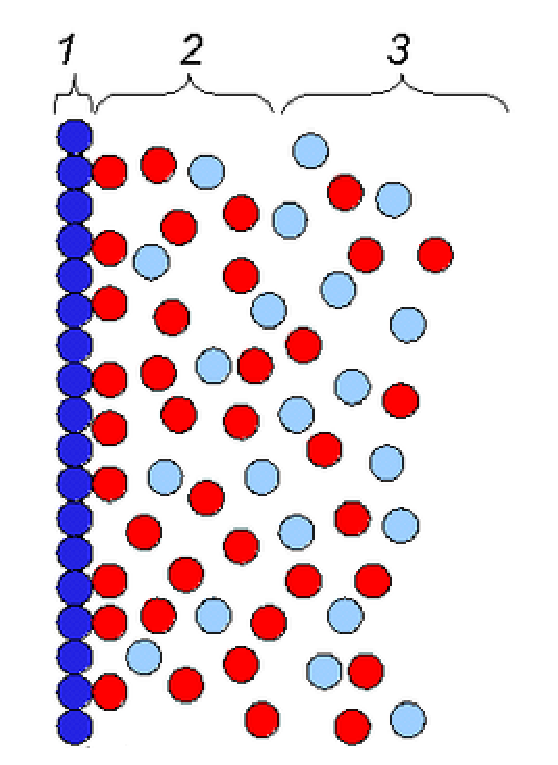
\includegraphics[width=0.25\textwidth]
            {ElectricDoubleLayer.eps}
        \caption{Schematic structure of the double layer:
        (1) particle's surface, (2) Debye layer and (3) fluid bulk.
        If the the particle's surface has positive (blue) surface charge, it attracts negative (red) ions from the fluid making the Debye layer be negatively charged (as opposed to the rest of the fluid bulk, which is electrically neutral).
        Zeta potential is defined as the voltage drop on (2).}
        \label{fig:EDL}
    \end{center}
\end{framed}
\end{figure}

In cases where the layer width is much smaller than the particle's size, an analytical solution for the Debye layer dynamics can be found \cite{Yariv10a}.

Electrokinetics is described by the following physical phenomena (in dimensionless formulation):
\begin{enumerate}
\item Electrostatic potential - the fluid bulk contains no free charge:
\begin{equation} \label{eq:Laplace}
    \bnabla \cdot (C \bnabla \varPhi) = 0.
\end{equation}
\item Fluid dynamics - Stokes incompressible flow with an electrostatic force component:
\begin{equation} \label{eq:Stokes}
\left\{ \begin{array}{l}
\bLaplacian \bV - \bnabla P + \Laplacian \varPhi \bnabla \varPhi = 0 \\
\bnabla \cdot \bV = 0 \end{array} \right.
\end{equation}
\item Ion diffusion and advection (via the fluid's velocity field):
\begin{equation} \label{eq:Nernst}
\Laplacian C - \alpha \bV \cdot \bnabla C = 0
\end{equation}
\end{enumerate}
The boundary conditions correspond to the specific problem at hand and defined by particle's geometry, chemical characteristics and fluid's dynamics.

The partial differential equations above are coupled and non-linear. In general, they have no analytic solution. Moreover, any numerical solver must handle the scale disparity, caused by the Debye layer width being much smaller than the particle's size.
A closed-form approximate solution has been developed for spherical ion-exchanging particles and small electric field \cite{Yariv10b} but it is hard to extend the analytic solution to more general systems.

\section{Research goals}
Our goal is to implement an accurate and fast iterative numerical solver for electrokinetic problems, which could be successfully applied for systems that have no closed-form solutions known (e.g. asymmetric particles or large electric fields).

The solver will be verified against known closed-form solutions for each of the sub-problems, as well as the full coupled problem, analyzing the discrepancies between the theoretical and numerical results.

Moreover, the convergence rate of the solver will be optimized using numerical acceleration methods in order to achieve high accuracy in reasonable execution time.

The solver will provide a numerical model for interesting electrokinetical phenomena which have no closed-form analytic solutions yet, such as large field dynamics and electrophoretic\footnote{Electrophoresis is the physical phenomenon of particles motion in an ion-containing fluid under the influence of an electric field.} autonomous micro-swimmers \cite{Paxton04, Howse07}.

\section{Achieved results}
The numerical solver is being implemented as a MATLAB package, which provides the needed tools for numerical solution of an electrophoresis problem.

The solver applies iterative relaxations to solve the coupled system, by
iterating the equations and relaxing each one of them
for the corresponding variable:
\begin{itemize}
  \item Laplace equation \ref{eq:Laplace} is used to update $\varPhi$.
  \item Stokes equation \ref{eq:Stokes} is used to update $\bV$ and $P$.
  \item Nernst-Planck equation \ref{eq:Nernst} is used to update for $C$.
\end{itemize}
While solving a specific equation for a specific variable, all other variables maintain their values from previous iteration, resembling ``Gauss-Seidel'' method for linear systems.

The problem's configuration is taken from \cite{Yariv10b} and consists of a spherical ion-exchanging particle, surrounded by infinite Stokes fluid.
Spherical coordinates $(R,\theta,\phi)$ system is chosen to make the problem axisymmetric, therefore independent of $\phi$.
The electrokinetic problem is written as two-dimensional partial differential equation system for $R \in [1,\infty)$ and $\theta \in [0, \pi]$.
Natural grid choices are a logarithmic grid for $R$ and an uniform grid for $\theta$.

The following linear operators are implemented in spherical coordinates on the grid described above: Scalar Laplacian (for $\varPhi$ and $C$), Vector Laplacian (for $\bV$), Gradient (for $\Phi, C$ and $P$) and Divergence (for $\bV$).
Each differential operator is written in spherical coordinates on the regular $(R, \theta)$ grid and being linear, is represented as a sparse matrix -- simplifying the algebraic manipulations.

The boundary conditions are defined for $\theta = 0$ and $\theta = \pi$ using symmetry considerations. At $R = \infty$, we assume constant fluid velocity $\bV = \cl{U} \bzhat$, constant electric field $\bnabla \varPhi = -\beta \bzhat$ and constant ionic concentration $C = 1$.
The boundary conditions on $R = 1$ are defined by the Debye layer's behavior as described in \cite{Yariv10b}, using the Dukhin-�Derjaguin slip formula for $\bV$ and ion-selectivity for $\varPhi$ and $C$.

After substitution of boundary conditions, each differential equation is transformed into a sparse linear system of the form $\matr{A}\bx = \vect{b}$.
Due to coupling, it is not necessary to find the exact solution -- so we apply few relaxations (\ref{eq:Relax}) on each linear system, using an appropriate preconditioner $\matr{M}_\matr{A}^{-1}$:
\begin{eqnarray} \label{eq:Relax}
  \bx_{n+1} &=& \bx_{n} + \matr{M}_\matr{A}^{-1} \left(\vect{b} - \matr{A}\bx_{n}\right)
\end{eqnarray}

After the solver has converged to a solution for the coupled system, the total stress tensor $\mathbb{T}$ on the particle $\cl{S} = \left\{\bx : \|\bx\| = 1\right\}$ is computed (\ref{eq:Stress}) and integrated to yield the total force (\ref{eq:Force}):
\begin{eqnarray}
  \label{eq:Stress}
  \mathbb{T} &=& - P \mathbb{I} + \bnabla \bV + (\bnabla \bV) ^T  + \bnabla \varPhi \bnabla \varPhi - \frac{\bnabla \varPhi \cdot \bnabla \varPhi}{2} \mathbb{I}, \\
  \label{eq:Force}
  \vect{F} &=& \int_{\cl{S}} \left(\mathbb{T} \cdot \bnhat \right) ds = \boldsymbol{0}.
\end{eqnarray}
Since the problem is axisymmetric, the force should be aligned with the symmetry axis: $\vect{F} = F \bzhat$.
Moreover, since the particle is stress-free in steady flow, we have $F = 0$ for steady-state velocity $\cl{U}$.

This observation enables us to find the correct $\cl{U}$ for given $\beta$, using one-dimensional root-finding algorithm on $F_\beta(\cl{U})$, as a function of $\cl{U}$.

The numerical solution for $\cl{U}$ as a function of $\beta$ is compared to the closed-form solution from \cite{Yariv10b}.
Using a $60 \times 15$ grid for $(R,\theta) \in [1, 100] \times [0, \pi]$, we apply $2\mathord{,}000$ iterations in order to find the total force acting on the particle.
This step is repeated a few times to find the correct $\cl{U}$ so that $F_\beta(\cl{U}) = 0$ for various $\beta$ values -- see Figure \ref{fig:Results} for numerical results.
\begin{figure}[htbp]
\begin{framed}
    \begin{center}
        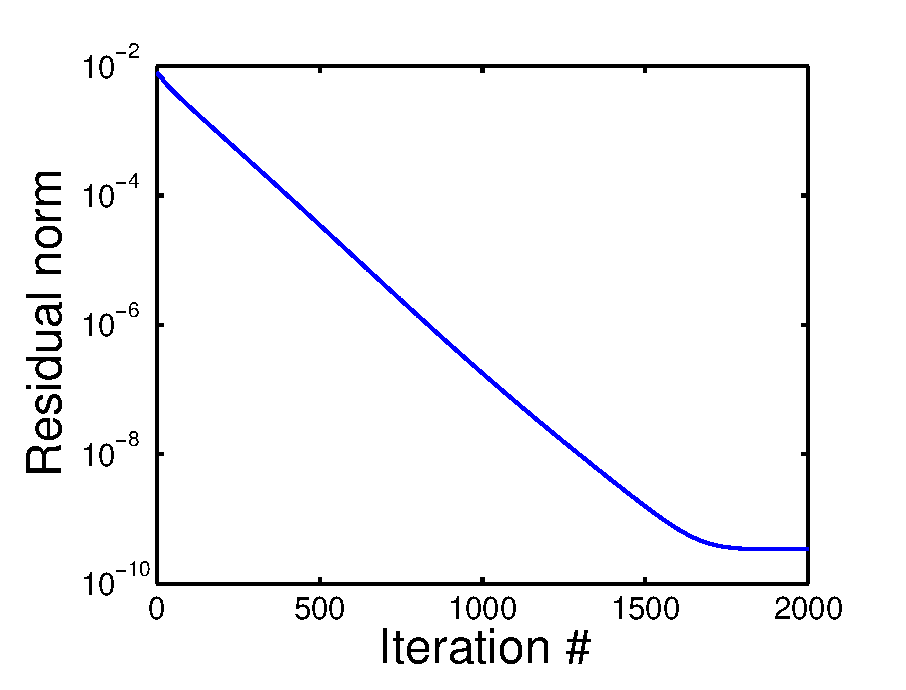
\includegraphics[width=0.45\textwidth]
            {convergence.eps}
        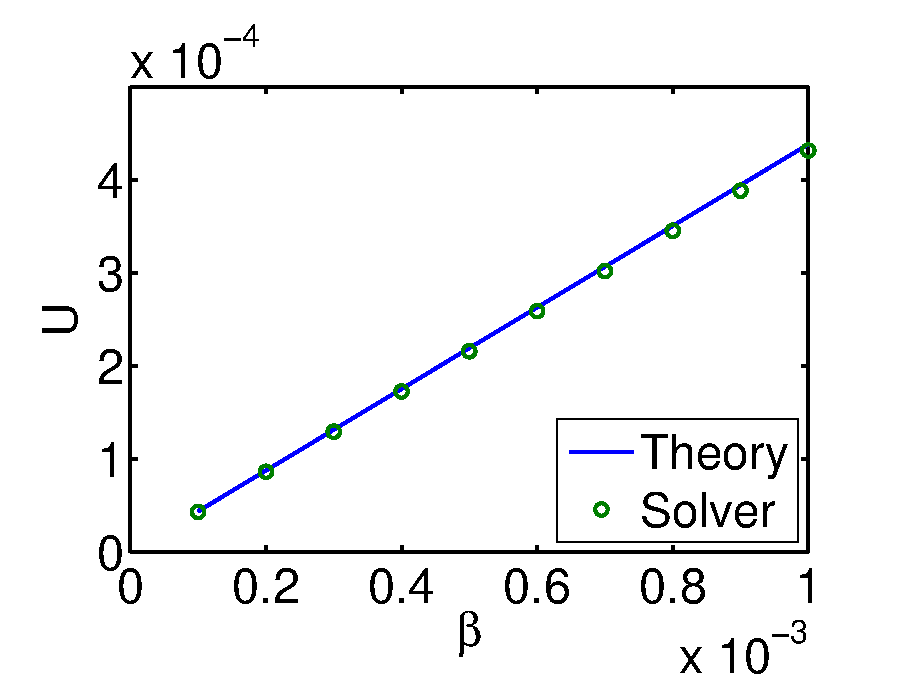
\includegraphics[width=0.45\textwidth]
            {comparison.eps}
        \caption{Left: Residual $\ell_2$ norm graph. Right: Particle Velocity $\cl{U}$ as a the function of electric field $\beta$.
        The error between the theoretical and the solver's results is less than 2\%.}
        \label{fig:Results}
    \end{center}
\end{framed}
\end{figure}

\section{Algorithms and techniques}

$C$, $\varPhi$ and $P$ are discretized using a central grid whereas a staggered grid is used for $\bV$ at the problem domain $\cl{D}$ (see Figure \ref{fig:Grids}).
\begin{figure}[htbp]
\begin{framed}
    \begin{center}
        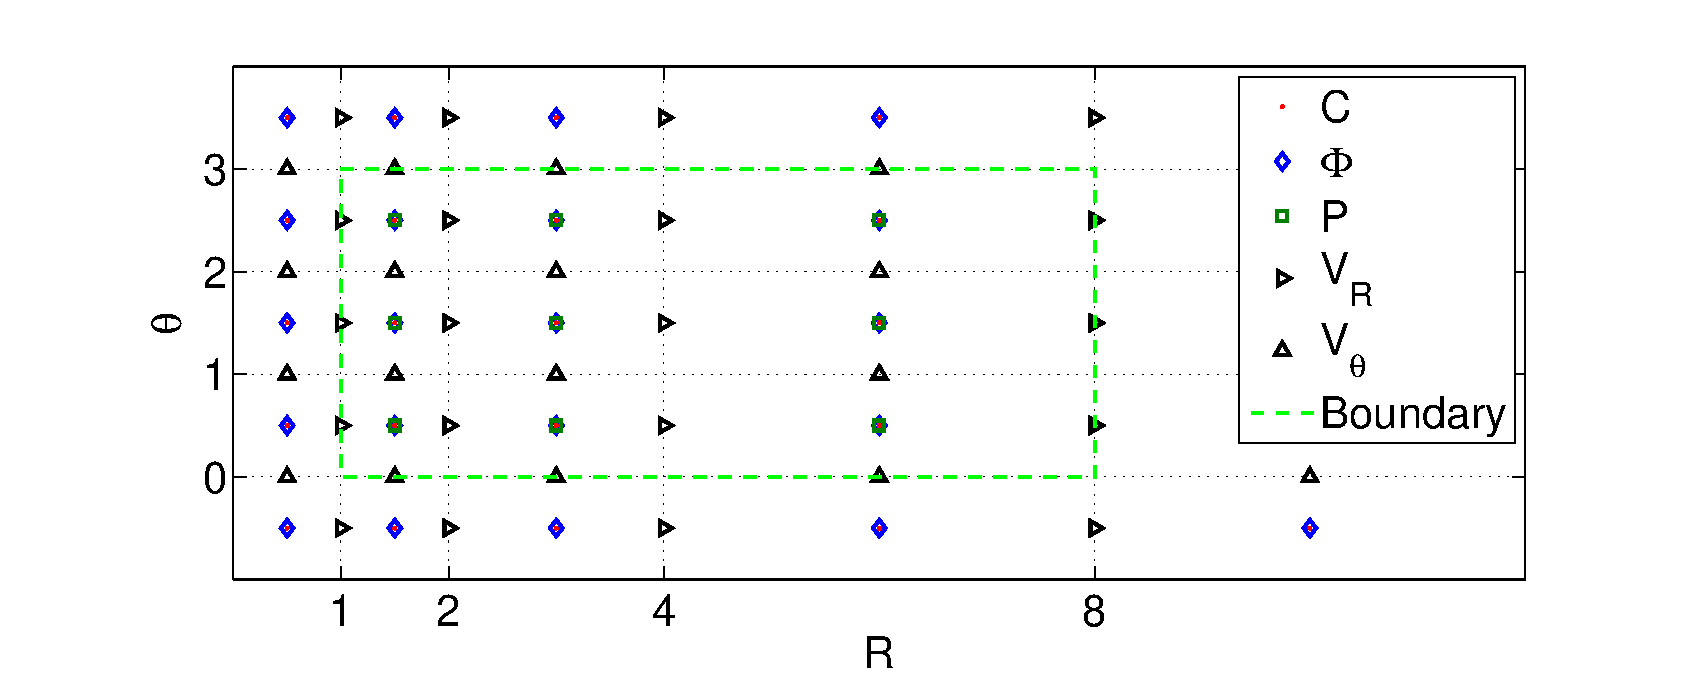
\includegraphics[width=1\textwidth]
            {StaggeredGrid.eps}
        \caption{Grids for $C$, $\varPhi$, $P$ and $\bV$.}
        \label{fig:Grids}
    \end{center}
\end{framed}
\end{figure}


Finite volume method is used to represent the partial differential equations in the form of an algebraic system, using central differences or an upwind scheme (for better stability).

``Ghost points'' are used to define Dirichlet and Neumann boundary conditions on
the problem domain's boundary $\partial \cl{D}$.

After boundary counditions are eliminated, Jacobi and Red-Black Gauss-Seidel preconditioners are used for equations \ref{eq:Laplace} and \ref{eq:Nernst}, where a Vanka-type \cite{Vanka86} preconditioner is used for equation \ref{eq:Stokes}.
The preconditioners are computed as sparse matrices, making the relaxations (at equation \ref{eq:Relax}) much more straightforward.

Vector extrapolation methods \cite{Sidi90} have been implemented and are used to accelerate the solver's convergence.
Multigrid solver \cite{Brandt77, Yavneh06} implementation will also be a part of the research.

\begin{thebibliography}{}
\bibitem{Yariv10a} E. Yariv,
``An asymptotic derivation of the thin-debye-layer limit for electrokinetic phenomena'',
{\em Chem. Engng Comm. 197, 3�17}, 2010.
\bibitem{Yariv10b} E. Yariv,
``Migration of ion-exchange particles driven by a uniform electric field'',
{\em Journal of Fluid Mechanics, 655 105-121}, 2010.
\bibitem{Rubin01} I. Rubinstein and B. Zaltzman,
``Electro-osmotic slip of the second kind and instability in concentration polarization at electrodialysis membranes'',
{\em Math. Mod. Meth. Appl. Sci. 11 (2), 263�300}, 2001.
\bibitem{Paxton04}
W. Paxton et. al.,
``Catalytic Nanomotors: Autonomous Movement of Striped Nanorods'',
{\em Journal of the American Chemical Society 126 (41), 13424-13431}, 2004.
\bibitem{Howse07}
J. R. Howse et. al.,
``Self-Motile Colloidal Particles: From Directed Propulsion to Random Walk'',
{\em Phys. Rev. Lett., 99, 048102}, 2007.
\bibitem{Vanka86}
S. P. Vanka,
``Block-implicit multigrid solution of Navier-Stokes equations in primitive variables'',
{\em J. Copmput. Phys., 65, 138-158}, 1986.
\bibitem{Sidi90}
A. Sidi, ``Efficient implementation of minimal polynomial and reduced rank extrapolation methods'',
{\em Journal of Computational and Applied Mathematics, Vol. 36, pp. 305-337}, 1991.
\bibitem{Brandt77} Achi Brandt,
``Multi-Level Adaptive Solutions to Boundary-Value Problems'',
{\em Mathematics of Computation, 31: 333�90}, 1977.
\bibitem{Yavneh06} Irad Yavneh.
``Why Multigrid Methods are so Efficient'',
{\em Computing in Science and Engineering, 8(6):12-22}, 2006
\end{thebibliography}

\end{document}
